%!TEX root =conext14.tex
\section{Performance Evaluation}
\label{sec:evaluation}

To evaluate the performance of our proposed system, we implemented our multipath IP in Ubuntu under Linux kernel $3.12.1$ and install the prototype on two desktops. Both desktops are connected directly to one router without any middlebox. At each desktop, two NICs working with $100Mbps$ capacity are installed which means that there are totally $4$ paths and the throughput upper bound is $200MBps$ between the two nodes. Also, to evaluate our prototype under multiple scenarios, for some experiments, we limit the capacity of one NIC card on the client to $30Mbps$ with built-in netem feature in Ubuntu. Also, we replace one NIC card on the client with a wireless NIC to evaluate our system for wireless environment.

Besides the controlled lab experiments, we also evaluate MPIP on the Internet. We connect the client to a customized node in Emulab. According to our test, the capacity between our client in the lab and the server in Emulab is about $5Mbps$, so we limit the bandwidth of both NICs on the client to be $2Mbps$. Because there is only one NIC that connects to Internet on the Emulab card, there are only $2$ paths in this case.

In all experiments, we try to keep the configuration of each node unchanged after installation. We don't any special configuration to the default TCP congestion control algorithm, neither we do any optimization to TCP parameters to squeeze out all possible throughput. Beside enabling MPIP feature at he kernel source tree, to make MPIP feasible, we need to configure IP routing rules to route incoming packets to a proper NIC as in MPTCP.

Except specific experiments that can only be applied to MPIP like UDP experiment and customization MPIP routing, we try to do side-by-side comparison with MPTCP for TCP connections. We will figure out how these two features work independently and together as stated in Section~\ref{sec:together};

For all throughput related experiments, we used iperf3 to transmit packets from the client to the server.

%We modify an open source software \bf{Simple Traffic Monitor}\cite{simon01} to record the real time traffic that goes through each NIC.

%For mobile devices, we implement this feature in Google Nexus $4$ with Android $4.01$.

\subsection{TCP/UDP throughput enhancement}
\label{sec:tcp}

In this section, we try to verify that our system can achieve high throughput in both TCP and UDP scenarios. 

In Figure~\ref{fig.nonat},

\begin{figure}[htb]
\centering{
\subfigure[TCP throughput with psudo TCP connection\label{fig.tcp_usetcp_nonat}]{\includegraphics[width=0.49\linewidth]{fig/tcp_usetcp_nonat.eps}}
\subfigure[TCP throughput with UDP Wrapper\label{fig.tcp_useudp_nonat}]{\includegraphics[width=0.49\linewidth]{fig/tcp_useudp_nonat.eps}}
}
\caption{Side-by-side comparison between different MPIP TCP implementations }
\label{fig.nonat}
\end{figure}


MPIP TCP uses fake TCP connection for all experiments below.

\begin{figure*}[htb]
\centering{
\subfigure[Throughput among MPIP, MPTCP and Together for no limit\label{fig.no_limitc}]{\includegraphics[width=0.24\linewidth]{fig/no_limit.eps}}
\subfigure[Delay among different paths for no limit\label{fig.delay_comp_no_limit}]{\includegraphics[width=0.24\linewidth]{fig/delay_comp_no_limit.eps}}
\subfigure[Queuing Delay among different paths for no limit\label{fig.queuing_delay_comp_no_limit}]{\includegraphics[width=0.24\linewidth]{fig/queuing_delay_comp_no_limit.eps}}
\subfigure[Throughput among different paths for no limit\label{fig.tp_comp_no_limit}]{\includegraphics[width=0.24\linewidth]{fig/tp_comp_no_limit.eps}}
}
\caption{Side-by-side comparison for no limit}
\label{fig.no_limit}
\end{figure*}


\begin{figure*}[htb]
\centering{
\subfigure[Throughput among MPIP, MPTCP and Together for limit\label{fig.limitc}]{\includegraphics[width=0.24\linewidth]{fig/limit.eps}}
\subfigure[Delay among different paths for limit\label{fig.delay_comp_limit}]{\includegraphics[width=0.24\linewidth]{fig/delay_comp_limit.eps}}
\subfigure[Queuing Delay among different paths for limit\label{fig.queuing_delay_comp_limit}]{\includegraphics[width=0.24\linewidth]{fig/queuing_delay_comp_limit.eps}}
\subfigure[Throughput among different paths for limit\label{fig.tp_comp_limit}]{\includegraphics[width=0.24\linewidth]{fig/tp_comp_limit.eps}}
}
\caption{Side-by-side comparison for limit}
\label{fig.limit}
\end{figure*}


\begin{figure*}[htb]
\centering{
\subfigure[Throughput among MPIP, MPTCP and Together for wireless\label{fig.wirelessc}]{\includegraphics[width=0.24\linewidth]{fig/wireless.eps}}
\subfigure[Delay among different paths for wireless\label{fig.delay_comp_wireless}]{\includegraphics[width=0.24\linewidth]{fig/delay_comp_wireless.eps}}
\subfigure[Queuing Delay among different paths for wireless\label{fig.queuing_delay_comp_wireless}]{\includegraphics[width=0.24\linewidth]{fig/queuing_delay_comp_wireless.eps}}
\subfigure[Throughput among different paths for wireless\label{fig.tp_comp_wireless}]{\includegraphics[width=0.24\linewidth]{fig/tp_comp_wireless.eps}}
}
\caption{Side-by-side comparison for wireless }
\label{fig.wireless}
\end{figure*}


\begin{figure*}[htb]
\centering{
\subfigure[out-of-order process\label{fig.outoforder}]{\includegraphics[width=0.33\linewidth]{fig/reorder.eps}}
\subfigure[Skype Audio Streaming Routing Adaptation\label{fig.skype}]{\includegraphics[width=0.33\linewidth]{fig/skype.eps}}
\subfigure[Connection Smooth Switch\label{fig.switch}]{\includegraphics[width=0.33\linewidth]{fig/switch.eps}}
}
\end{figure*}


\subsection{Out-of-order evaluation for TCP}
\label{sec:reoder}

To evaluation the effect of out-of-order process in our prototype, we design following experiment. We replace one NIC with wireless NIC, then there will still be $4$ paths. For all the paths, we assign the same path weight which means that every path is assigned the same amount of packets. In this scenario, $50\%$ percent of packets will be sent throughput the wireless NIC. The difference between propagation delay of the wireless path and wired path is large enough to generate a substantial number of out-of-order packets. By enabling and disabling out-of-order functionality, we get Figure~\ref{fig.outoforder}.


\subsection{Skype voice call improvement}
\label{sec:skype}

In Section~\ref{sec:resp}, we mentioned that 
In Figure~\ref{fig.skype}, we prove that our packet-size based routing decision works perfectly for audio application like Skype. In our experiment, we change the delay of NIC cards using the netem package in Ubuntu. On one side of the Skype call, we have two NIC cards as stated above. We ran the experiment for $360$ seconds with $3$ sections. In the first $120$ seconds, there is no manually added delay on each NIC card, we add additional $120ms$ delay to the first NIC card in the following $120$ seconds, finally for the last $120$ seconds, we add $120ms$ delay to the second NIC card. We did our Skype audio experiment without video content while most packets on the connection are audio packets except some control packets.The size of Audio packets is relative small, generally under $200$KB. In this case, according to Equation~\ref{eq.bw} to Equation~\ref{eq.c}, the routing decision will mostly depend on the delay value instead of queuing delay. Figure~\ref{fig.skype} shows the packets routing adaptation as the delay value changes. By this adaptation, we can make sure that the audio streaming will always choose the path that has lower delay to keep the best user experience even other paths have the same throughput.


\subsection{Smooth connection switch}
\label{sec:switch}

In Figure~\ref{fig.switch}, we verify that smooth switch between different NIC cards works perfectly over our MPIP implementation by doing an IPERF TCP experiment. We do a side-by-side comparison between MPIP and MPTCP. We also divide the experiment into $3$ sections with $120$ seconds for each section. On the client side of the connection, there are two NIC cards. In the first $120$ seconds, both NIC cards work synchronously, then we disable one of them for $120$ seconds, and during the last $120$ seconds, we enable back the NIC card. The result shows that our MPIP system can follow this on/off process perfectly with stable throughput. For MPTCP, as shown in previous experiments, MPTCP has higher fluctuation than MPIP even MPTCP can achieve higher throughput than MPIP. This happens because in MPTCP, there are more than one TCP connections ($4$ in this experiment), and each connection has its own congestion window. Although congestion control in MPTCP is coupled among different connections, fluctuation have more chances to happen with $4$ relatively independent congestion windows. But in MPIP, one one TCP connection is constructed for each session which means that there is only one congestion windows. In this case, the throughput is more consistent than that of MPTCP.